\documentclass{article}
\usepackage{amsmath, amssymb, tikz, geometry, graphicx, natbib, mwe, color, xcolor, listings, tabularx, pdfpages, blindtext, mathtools, stackengine, pgfplots,bigints, relsize, upgreek, esint, array, multirow, schemata, wrapfig, cancel, comment, svg}
\usepackage{hyperref}
\usepackage{slashed, enumitem}
\usepackage{titlesec}
\usetikzlibrary{positioning}

\begin{comment}
code to write section, subsection and subsubsection title in a specific color
\titleformat{\section}
{\color{synthwave_text}\normalfont\Large\bfseries}
{\color{synthwave_text}\thesection}{1em}{} 

\titleformat{\subsection}
{\color{synthwave_text}\normalfont\large\bfseries}
{\color{synthwave_text}\thesubsection}{1em}{} 

\titleformat{\subsubsection}
{\color{synthwave_text}\normalfont\normalfont\bfseries}
{\color{synthwave_text}\thesubsubsection}{1em}{}
\end{comment}


\pgfplotsset{compat=1.9}

\colorlet{myWhite}{white!35!gray}
\definecolor{shadeofgray}{HTML}{181818}
\definecolor{shadeofviolet}{HTML}{0f022c}
\definecolor{synthwave_beckground}{HTML}{252334}
\definecolor{synthwave_text}{HTML}{e148aa}


\hypersetup{
    colorlinks=true,
    linkcolor=violet,
    filecolor=magenta,      
    urlcolor=cyan,
    pdftitle={Tecnologie Web T},
    pdfpagemode=FullScreen,
}


\geometry{ 
 a4paper,
 left=10mm,
 right=10mm,
 top=10mm
 }
 
\lstdefinestyle{mystyle}{ 
bracketsstyle=\color{red}
}

\title{Tecnologie Web T}
\author{Giuseppe Bumma}


% color option
%\pagecolor{synthwave_beckground} %{shadeofgray}
%\color{myWhite}

\renewcommand{\CancelColor}{\color{synthwave_text}}


\begin{document}

%Commands
\newcommand{\R}{\mathbb{R}}
\newcommand{\Varepsilon}{\mathcal{E}}
\newcommand{\rad}{\text{rad}}
\newcommand{\bb}[1]{\mathbb{#1}}
\newcommand{\cc}[1]{\mathcal{#1}}
\newcommand{ \lognormal }{\text{Lognormal} }
\newcommand{\T}[1]{\text{#1}}
\newcommand*\circled[1]{\tikz[baseline=(char.base)]{%
            \node[shape=circle,draw,inner sep=2pt] (char) {#1};}}
%for using circled number in enumerate use:
%\begin{enumerate}[label=\protect\circled{\arabic*}]


\tableofcontents

\maketitle

\section{Introduzione}
Il World Wide Web (WWW) è stato proposto nel 1989 da Tim
Berners-Lee, ricercatore di fisica al CERN di Ginevra.\\
L'idea alla base del progetto era quella di fornire
strumenti adatti a condividere:
\begin{itemize}
    \item documenti statici
    \item in forma ipertestuale
    \item disponibili su rete Internet tramite protocollo
    semplice e leggero
\end{itemize}
Si volevano rimpiazzare i sistemi di condivisione di documenti basati su protocolli più vecchi come FTP e Gopher.
\subsection{Storia}
\begin{itemize}
    \item Nel marzo del 1989 Tim Berners-Lee
    elaborò una proposta
    \item Il 12 novembre 1990 assieme a Robert
    Cailliau presentò una proposta più
    formale per un sistema ipertestuale
    basato su un'architettura client-server
    \item Il 6 agosto 1991 Berners-Lee mise
    on-line su Internet il primo sito Web
    Inizialmente fu utilizzato solo dalla
    comunità scientifica
    \item Il 30 aprile 1993 il CERN decise di
    rendere pubblica la tecnologia alla
    base del Web
\end{itemize}
L'HTTP (\textbf{HyperText Transfer Protocol}) è un protocollo che sta alla base dell'internet e che permette lo scambio di informazioni in architetture client-server. Ci sono state varie implementazioni del protocollo HTTP
\begin{itemize}
    \item HTTP/1.0, implementato nel 1991 e
    proposto come Request for Comment
    RFC 1945 a Internet Engineering Task
    Force IETF nel 1996
    \item HTTP/1.1, presentato come RFC
    2068 nel 1997 e aggiornato/approvato
    nel 1999 come RFC 2616
    \item HTTP/2 (origin. chiamato HTTP/2.0),
    basato su SPDY, sviluppato dal Working
    Group Hypertext Transfer Protocol
    (httpbis) di IETF
    \item HTTP/2 pubblicato come RFC 7540 a Maggio 2015, 63\% circa del traffico secondo le ultime statistiche
\end{itemize}



\subsection{Gli ipertesti}
Un \textbf{ipertesto} (hypertext) è un insieme di documenti messi in relazione tra loro tramite collegamenti monodirezionali (hyperlink o più semplicemente link). Può essere visto come una rete (un
grafo) e i documenti ne costituiscono i nodi.
\begin{center}
    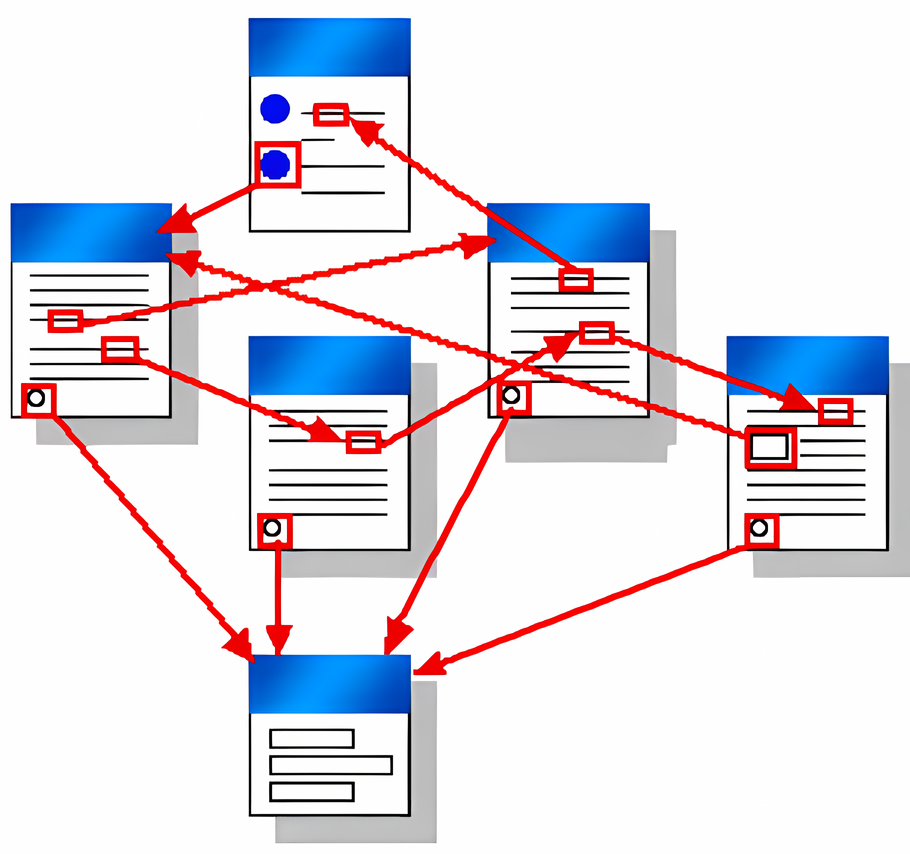
\includegraphics[scale=0.17]{Images/Ipertesto.png}
\end{center}
Attraverso un link possiamo passare da un
punto di un documento ad un altro qualunque dei documenti del grafo. La caratteristica principale di un ipertesto è che la lettura può svolgersi in maniera non lineare: qualsiasi documento della rete può essere il successivo.\\
Se si prendono in considerazione non solo testi ma elementi multimediali (immagini suoni, video) si parla di ipermedia.


\subsection{WWW come sistema ipertestuale}
Idea (e motivazione di successo) di Berners-Lee è stata quella di mettere insieme le idee di ipertesto e rete Internet in modo efficace. World Wide Web è in pratica un ipertesto distribuito sulla rete in cui i documenti, chiamati anche pagine, risiedono su server geograficamente distribuiti (World Wide) e costituiscono una ragnatela virtuale (Web). Da un qualunque documento è possibile “saltare” ad un altro indipendentemente da dove questo si trovi.
\vspace*{0.2cm}\\
Per realizzare questo ipertesto planetario abbiamo
bisogno di tre elementi concettuali:
\begin{itemize}
    \item un meccanismo per localizzare un documento     
    \item un protocollo per accedere alle risorse che costituiscono il documento e trasferirle al client
    \item un linguaggio per descrivere i documenti ipertestuali (usato per costruire le pagine)
\end{itemize}
e di due elementi fisici:
\begin{itemize}
    \item un server in grado di erogare le risorse che costituiscono i documenti
    \item Un client in grado di rappresentare/visualizzare i documenti e di consentire la navigazione da un documento all'altro
\end{itemize}



\subsection{Elementi del Web}
In estrema sintesi nella sua visione iniziale il Web può essere rappresentato con la “formula”:
\begin{center}
    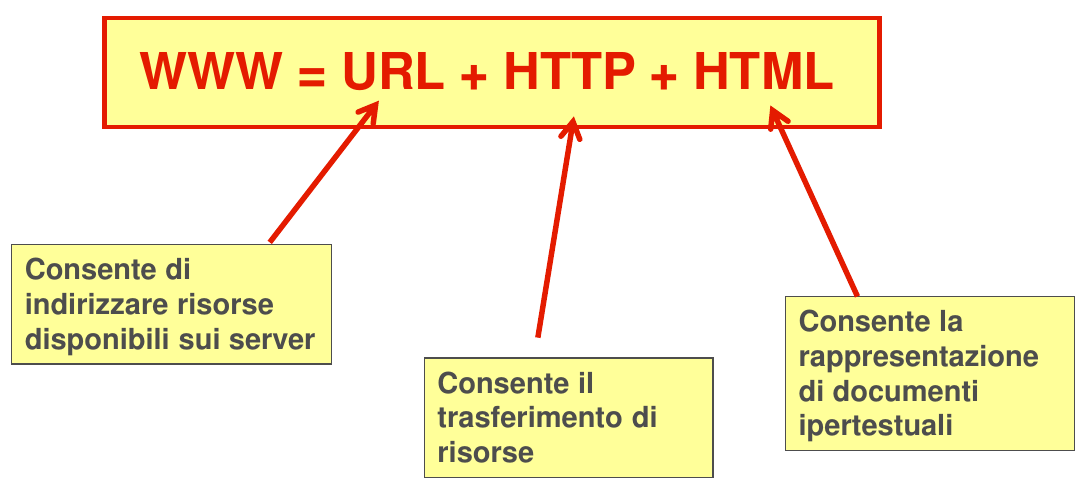
\includegraphics[scale=0.27]{Images/Formula_web.png}
\end{center}
Il Web segue un modello Client/Server: i client \textbf{attivi}, detti Web Browser utilizzano il protocollo HTTP per connettersi ai server; i server \textbf{passivi}, detti Web o HTTP Server rimangono in ascolto di eventuali connessioni di nuovi client, utilizzano il protocollo HTTP per interagire con i client e forniscono ai client le pagine Web che questi richiedono.


\section{URI e URL}
\subsection{URI}
\subsubsection{Problematiche fondamentali}
L'URL (primo componente della formula del Web) fa riferimento a tre questioni principali:
\begin{itemize}
    \item come identificare il server in grado di fornirci un elemento dell'ipertesto
    \item come identifichiamo la risorsa a cui vogliamo accedere?
    \item quali meccanismi (ad es. in termini di protocollo) possiamo utilizzare per accedere alla risorsa?
\end{itemize}
La risposta a tutte queste domande sono gli URI.


\subsubsection{Cosa sono}
Gli URI (Uniform Resource Identifier) forniscono un meccanismo semplice ed estensibile per identificare una risorsa. Con il termine risorsa intendiamo qualunque entità abbia una identità: un documento, un'immagine, un servizio, una collezione di altre risorse.
\vspace*{0.2cm}\\
Un URI è un \textbf{concetto generale}, quindi non fa riferimento solo a risorse alle quali si può accedere con protocollo HTTP o a entità disponibili in rete. Si dice che è un \textbf{mapping} concettuale a una identità, e non si riferisce a una particolare versione dell'entità esistente in un dato momento. Il mapping può rimanere inalterato anche se cambia il contenuto della risorsa.


\subsubsection{Sintassi}
Gli URI rispettano una sintassi standard, semplice e regolare:
\begin{verbatim}
    URI = scheme ":" ["//" authority] path ["?" query] ["#" fragment]
\end{verbatim}
\begin{center}
    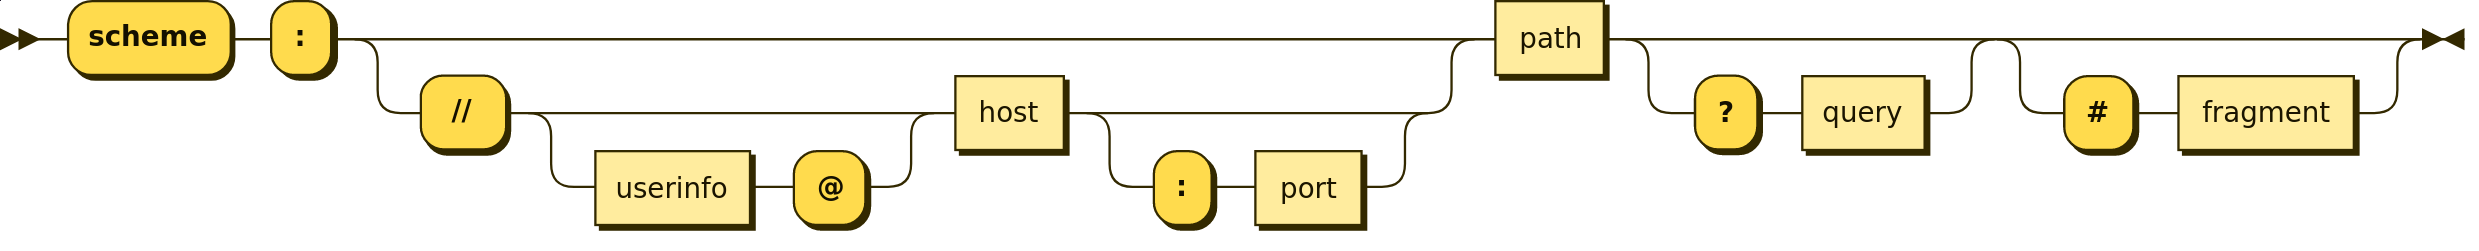
\includegraphics[scale=0.19]{Images/URI_diagram.png}
\end{center}


\subsection{Specializzazioni di URI: URN e URL}
Esistono due specializzazioni del concetto di URI:
\begin{itemize}
    \item Uniform Resource Name (URN): identifica una risorsa per mezzo di un “nome” che deve essere globalmente unico e \textbf{restare valido anche se la risorsa diventa non disponibile} o cessa di esistere
    \item Uniform Resource Locator (URL): identifica una risorsa per mezzo del suo \textbf{meccanismo di accesso primario} (es. locazione nella rete) piuttosto che sulla base del suo nome o dei suoi attributi
\end{itemize}
Applicando questi concetti ad una persona: l'URN è come identificazione basata su
nome+cognome, o meglio codice fiscale, quindi io conosco quella persona ma non so dov'è, l'URL è come indirizzo di casa o numero di telefono (se univoci).



\subsection{URN}
Un URN identifica una risorsa mediante un nome in un particolare dominio di nomi (namespace), quindi consente di "parlare" di una risorsa prescindendo dalla sua ubicazione e dalle modalità con cui è possibile accedervi.\\
Un esempio molto noto è il codice ISBN (International Standard Book Number) che identifica a livello internazionale in modo univoco e duraturo un libro o una dizione di un libro di un determinato editore.


\subsection{URL}
Un URL tiene conto anche della modalità per accedere alla risorsa, infatti specifica il protocollo necessario per il trasferimento della risorsa stessa (tipicamente il nome dello schema corrisponde al protocollo utilizzato).\\
Nella sua forma più comune (schema HTTP-like) sintassi è
\begin{verbatim}
    <protocol>://[<username>:<password>@] <host>[:<port>][/<path>[?<query>][#fragment]]
\end{verbatim}
Questa forma vale per diversi protocolli di uso comune come HTTP, HTTPS, FTP, WAP, etc ...


\subsubsection{Compobenti di un URL}
Vediamo ora le componenti di un indirizzo URL nel dettaglio:
\begin{itemize}
    \item {\fontfamily{lmtt}\selectfont <protocol>}: descrive il protocolo da utilizzare per l'accesso al server
    \item {\fontfamily{lmtt}\selectfont <username>:<password>@}: credenziale per l'autenticazione (oggigiorno non si usano mai perché non è sicuro inserirle nell'URL)
    \item {\fontfamily{lmtt}\selectfont <host>}: indirizzo server su cui risiede la risorsa; può essere un indirizzo logico o fisico
    \item {\fontfamily{lmtt}\selectfont <path>}: percorso (\textit{pathname}) che identifica la risorsa nel file system del server; se manca, tipicamente di accede alla home page 
    \item {\fontfamily{lmtt}\selectfont <query>}: una stringa di caratteri che consente di passare al server uno o più parametri; di solito ha questo formato:
    \begin{verbatim}
        parametro1=valore&parametro2=valore2...
    \end{verbatim}
\end{itemize}
Esempio di URL con schema HTTP:
\begin{center}
    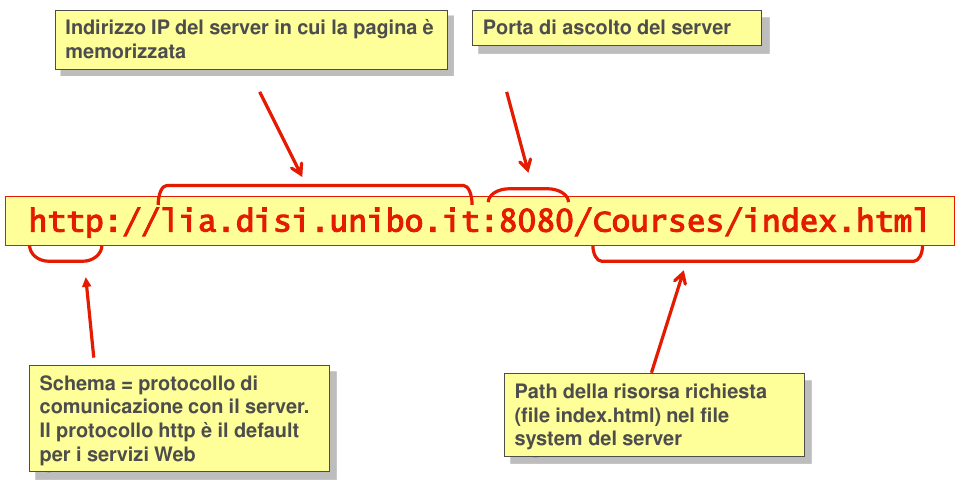
\includegraphics[scale=0.27]{Images/Es_URL.png}
\end{center}


\subsection{URI opache e gerarchiche}
Le URI possono essere anche classificate come opache o gerarchiche
\begin{itemize}
    \item l'URI opaca non è soggetta a ulteriori operazioni di \textbf{\textit{parsing}}; esempio
    \begin{verbatim}
        mailto:paolo.rossi@disi.unibo.it
    \end{verbatim}
    \item L'URI gerarchica è soggetta a ulteriori operazioni di parsing, per esempio per separare l'indirizzo del server dal percorso all'interno del file system; alcuni esempi:
    \begin{verbatim}
        http://informatica.unibo.it/
    \end{verbatim}
    qui non è specificato un path, quindi il server ritorna la home page identificata dal file {\fontfamily{lmtt}\selectfont index.html}
    \begin{verbatim}
        docs/guide/collections/designfaq.html#28
        ../../../lab/examples/ant/build.xml
    \end{verbatim}
    i {\fontfamily{lmtt}\selectfont ".."} indicano il server che sto visitando in quel momento
    \begin{verbatim}
        file:///~/calendar
    \end{verbatim}
\end{itemize}


\subsubsection{Operazioni sulle URI gerarchiche}
Di seguito si elencano le operazioni possibili su URI gerarchiche:
\begin{itemize}[label=$\blacktriangleright$]
    \item \textbf{Normalizzazione:} processo di rimozione dei segmenti {\fontfamily{lmtt}\selectfont "."} e {\fontfamily{lmtt}\selectfont ".."} (e altri caratteri speciali) dal path (N.B. la normalizzazione si applica solo a URI gerarchiche, su URI opache non ha effetto)
    \item \textbf{Risoluzione:} processo che a partire da una URI originaria porta all'ottenimento di una URI risultante; la URI originaria viene risolta basandosi sulla base URI
    \item \textbf{Relativizzazione:} processo inverso all risoluzione
\end{itemize}
Esempio di risoluzione di una URI:\\
URI originaria:
\begin{verbatim}
    docs/guide/collections/designfaq.html#28
\end{verbatim}
Base URI:
\begin{verbatim}
    http://disi.unibo.it/
\end{verbatim}
Risultato:
\begin{verbatim}
    http://disi.unibo.it/docs/guide/collections/designfaq.html#28
\end{verbatim}






















































\end{document}